\documentclass[UTF8]{ctexart}
\title{实验报告模板}
\usepackage{ctex}
\usepackage{multirow}
\usepackage{tabularx}
\usepackage{xcolor}
\usepackage{graphicx}
\usepackage{amsmath}
\usepackage{fancyhdr}
\usepackage{listings}
\usepackage{makecell}
\usepackage{caption}
\usepackage{threeparttable}
\usepackage{pdfpages}
\usepackage{appendix}
\usepackage{bookmark}
\usepackage{hyperref}
\usepackage[capitalise]{cleveref}%解决跳转不正确的问题
\lstset{
	basicstyle = \sffamily, % 基本代码风格 
	keywordstyle = \color{red}\bfseries, % 关键字风格 
	commentstyle = \color{blue}\rmfamily\itshape, % 注释的风格,斜体 
	stringstyle = \ttfamily, % 字符串风格 
	flexiblecolumns, % 别问为什么,加上这个 
	numbers = left, % 行号的位置在左边 
	showspaces = true, % 是否显示空格,显示了有点乱,所以不现实了 
	numberstyle = \zihao{-4}\ttfamily, % 行号的样式,小五号,tt等宽字体 
	showstringspaces = false,
	captionpos = t, % 这段代码的名字所呈现的位置,t指的是top上面 
	frame = single, % 显示边框
}
\lstdefinestyle{Python}{
	language = Python, % 语言选Python 
	basicstyle = \zihao{-5}\ttfamily,
	numberstyle = \zihao{-5}\ttfamily,
	keywordstyle = \color{blue},
	keywordstyle = [2] \color{teal},
	stringstyle = \color{magenta},
	commentstyle = \color{red}\ttfamily,
	breaklines = true, % 自动换行,建议不要写太长的行 
	columns = fixed, % 如果不加这一句,字间距就不固定,很丑,必须加 
	basewidth = 0.5em,	
	showstringspaces=false,
	frame=single,
}

\usepackage[a4paper,top=2.5cm,bottom=2cm,left=2cm,right=2cm,marginparwidth=1.75cm]{geometry}
\ctexset{
	section={
		format+=\zihao{-4}  \raggedright \textbf{} \fbox,
		name={},
		number={},
		beforeskip = 1.0ex plus 0.2ex minus .2ex,
		afterskip = 1.0ex plus 0.2ex minus .2ex,
		aftername=
	},
	subsection={
		format+=\zihao{-4}  \raggedright \textbf{} ,
		name={,、},
		number=\chinese{subsection},
		beforeskip = 1.0ex plus 0.2ex minus .2ex,
		afterskip = 1.0ex plus 0.2ex minus .2ex,
		aftername=
	}
}
\usepackage{hyperref}
\hypersetup{hypertex=true,
	colorlinks=true,
	linkcolor=black,
	anchorcolor=black,
	citecolor=black}
\pagestyle{fancy}
\fancyhf{}
\cfoot{\thepage}

\newcommand\tit{实验E4 晶体电光、声光和磁光效应}
\newcommand\head[1]{\fancyhead[L]{\kaishu 中山大学物理与天文学院近代物理实验\uppercase\expandafter{\romannumeral2} #1 }}
\fancyhead[R]{\kaishu \tit}
\newcommand\degree{^\circ}
\newcommand\dotpar[1]{$\bullet$ #1 \par}
\newcolumntype{Y}{>{\centering\arraybackslash}X}

%%插入单张图片
\newcommand{\singlefig}[4]{
	\begin{figure}[!h]
		\centering
		\includegraphics[width=#4\textwidth]{#1}
		\caption{#2}
		\label{#3}
	\end{figure}
}

\begin{document}

\begin{center}
	\renewcommand\arraystretch{2}
\begin{tabularx}{\textwidth}{|Y|Y|Y|Y|Y|Y|Y|Y|}
\hline 
\multicolumn{2}{|c|}{\textbf{\large 预习报告}}&\multicolumn{2}{c|}{\textbf{\large 实验记录}}&\multicolumn{2}{c|}{\textbf{\large 分析讨论}}&\multicolumn{2}{c|}{\textbf{\large 总成绩}}\\ \hline
 & & & & & & & \\ \hline

\end{tabularx}
\end{center}
\begin{center}
	\renewcommand\arraystretch{1.5}
	\begin{tabularx}{\textwidth}{|l|Y|l|Y|}
	\hline 
	年级、专业:&19级物理学&组号:&\\ \hline
	姓名:&刘耿昊&学号:&19342070\\ \hline
	日期:&\today&教师签名:& \\
	\hline
\end{tabularx}
\end{center}
\vspace{5pt}
\begin{center}
	\Large
	\textbf{\tit}
\end{center}
\head{预习报告}
\section{实验报告注意事项}
\begin{enumerate}
	\item 实验报告由三部分组成:
	\begin{itemize} 
		\item 预习报告:(提前一周)认真研读实验讲义,弄清实验原理;实验所需的仪器设备、用具及其使用(强烈建议到实验室预习),完成课前预习思考题;了解实验需要测量的物理量,并根据要求提前准备实验记录表格(第一循环实验已由教师提供模板,可以打印)。预习成绩低于10分(共20分)者不能做实验。
		\item 实验记录:认真、客观记录实验条件、实验过程中的现象以及数据。实验记录请用珠笔或者钢笔书写并签名\textcolor{red}{(用铅笔记录的被认为无效)。保持原始记录,包括写错删除部分,如因误记需要修改记录,必须按规范修改。}(不得输入电脑打印,但可扫描手记后打印扫描件);离开前请实验教师检查记录并签名。
		\item 分析讨论:处理实验原始数据(学习仪器使用类型的实验除外),对数据的可靠性和合理性进行分析;按规范呈现数据和结果(图、表),包括数据、图表按顺序编号及其引用;分析物理现象(含回答实验思考题,写出问题思考过程,必要时按规范引用数据);最后得出结论。

	\end{itemize}
		实验报告就是将预习报告、实验记录、和数据处理与分析合起来,加上本页封面。
\item 每次完成实验后的一周内交实验报告(特殊情况不能超过两周)。
\item 除实验记录外,实验报告其他部分建议双面打印。
\end{enumerate}

\newpage
\begin{center}
	\Large
	\textbf{\tit}
\end{center}
\section{实验目的}
\begin{center}
	\large \textbf{实验1 晶体的电光效应实验}
\end{center}
\begin{enumerate}
	\item 掌握晶体电光调制的原理和实验方法;
	\item 了解一种激光通信的方法
\end{enumerate}

\section{仪器用具}
\begin{figure}[!h]
	\centering
	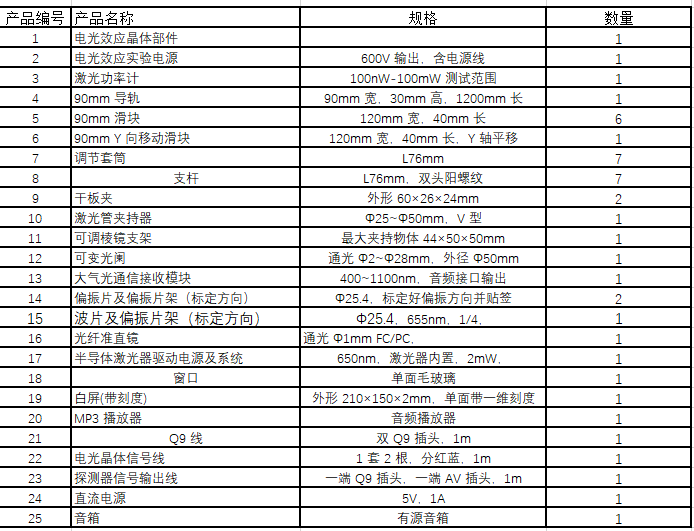
\includegraphics[width=0.9\textwidth]{tab}
\end{figure}
\section{实验原理}
\subsection{一次电光效应}
由电场所引起的晶体折射率变化称为电光效应。可以表示为:
\begin{equation}
	n=n_{0}+aE_{0}+bE_{0}^{2}+...
\end{equation}
一次项所引起的折射率变化即为一次电光效应

一次电光效应只存在于不具有对称中心的晶体中。

一次效应要比二次效应更显著。

\subsection{折射率椭球}

光在各向异性晶体中传播时折射率会因传播方向改变而变化,可以将折射率与光传播方向、振动方向表示为折射率椭球:
\begin{equation}
	\frac{x^{2}}{n_{1}^{2}}+\frac{y^{2}}{n_{2}^{2}}+\frac{z^{2}}{n_{3}^{2}}=1
\end{equation}

加上电场后,各向异性产生,则折射率变为:
\begin{equation}
	\frac{x^{2}}{n_{11}^{2}}+\frac{y^{2}}{n_{22}^{2}}+\frac{z^{2}}{n_{33}^{2}}+\frac{2 y z}{n_{23}^{2}}+\frac{2 x z}{n_{13}^{2}}+\frac{2 x y}{n_{12}^{2}}=1
\end{equation}
有两种一次电光效应:
\begin{enumerate}
	\item 纵向电光效应:电场方向与传播方向平行时产生。如KD*P类型晶体
	\item 横向电光效应:电场方向与传播方向垂直时产生。如LiNbO3晶体
\end{enumerate}
本实验研究铌酸锂晶体的一次电光效应,用铌酸锂晶体的横向调制装置测量铌酸锂晶体的
半波电压及电光系数,并用两种方法改变调制器的工作点,观察相应的输出特性的变化。

\singlefig{1}{}{}{0.8}
\subsection{电光调制原理}
激光作为高频载波,信号多调制于其强度上,也可以采用连续调幅、调频、调相以及脉冲调制等形式。强度调制是根据
光载波电场振幅地平方比例调制信号。

原因:光接收器一般都是直接相应其所接受的光强度变化。

方法:机械调制、电光调制、声光调制、磁光调制、电源调制等

电光调制开算速度快、结构简单。电光调制根据所施加的电场方向的不同,可分为纵向电光调制和横向电光调制。
\subsubsection{铌酸锂晶体横调制}
\singlefig{2}{横调制器}{tzq}{0.6}
\begin{equation}
	\Gamma \sim \frac{LV}{d}
\end{equation}
铌酸锂晶体具有优良的加工性能及很高的电光系数, 
$\gamma_{22}=6.8 \times 10^{-12} \mathrm{~m} / \mathrm{V}$, 
常常用来做成横向调制器, 铌酸锂为单轴晶体, 有 $n_{x}=n_{y}=n_{0}=2.286, n_{z}=n_{e}=2.203$

把晶体的通光方向设为 Z 方向,沿 X 方向施加电场E。晶体由单轴变为双轴,
新的主轴 $X^{'},Y^{'},Z^{'}$轴又称为感应轴,其中$X^{'},Y^{'}$绕 Z 轴转 45°,而 $Z^{'}$与 Z 轴重
合。晶体的线性电光系数$\gamma$是一个三阶张量,受晶体对称性的影响,铌酸锂的线
性电光系数矩阵为
\begin{equation}
	\gamma=\left[\begin{array}{ccc}
	0 & -\gamma_{22} & \gamma_{13} \\
	0 & \gamma_{22} & \gamma_{13} \\
	0 & 0 & \gamma_{33} \\
	0 & \gamma_{42} & 0 \\
	\gamma_{42} & 0 & 0 \\
	-\gamma_{42} & 0 & 0
	\end{array}\right]
	\end{equation}
施加电场后,得到电场强度矩阵(E,0,0),此时在 X 轴上加上电场后的电光系数矩阵为
\begin{equation}
	\left[\begin{array}{l}
	\Delta B_{1} \\
	\Delta B_{2} \\
	\Delta B_{3} \\
	\Delta B_{4} \\
	\Delta B_{5} \\
	\Delta B_{6}
	\end{array}\right] \equiv\left[\begin{array}{ccc}
	0 & -\gamma_{22} & \gamma_{13} \\
	0 & \gamma_{22} & \gamma_{13} \\
	0 & 0 & \gamma_{33} \\
	0 & \gamma_{42} & 0 \\
	\gamma_{42} & 0 & 0 \\
	-\gamma_{22} & 0 & 0
	\end{array}\right]\left[\begin{array}{c}
	E \\
	0 \\
	0
	\end{array}\right] \equiv\left[\begin{array}{c}
	0 \\
	0 \\
	0 \\
	0 \\
	\gamma_{42} E \\
	-\gamma_{22} E
	\end{array}\right]
	\end{equation}
当外加电场(E,0,0)时,电场作用下的光折射率椭球方程为
\begin{equation}
	\frac{x^{2}}{n_{0}^{2}}+\frac{y^{2}}{n_{0}^{2}}+\frac{z^{2}}{n_{e}^{2}}+2 \gamma_{42} E_{x z}+2 \gamma_{22} E_{x y}=1
\end{equation}
沿 Z 轴方向射入入射光,令上式的 Z=0,折射率椭球就变为与波矢
垂直的折射率平面,如图 1-3 所示为加了电场后的折射率椭球截面图,经过坐标
转换,得到截迹方程为:
\begin{equation}
	\left(\frac{1}{n_{0}^{2}}-\gamma_{22} E\right) x^{\prime 2}+\left(\frac{1}{\mathrm{n}_{0}^{2}}+\gamma_{22} \mathrm{E}\right) \mathrm{y}^{\prime 2}=1
	\end{equation}
\newpage
%\singlefig{page4-88}{沿x轴方向施加电场后的折射率椭球}{}{0.3}
故新主轴折射率为:
\begin{equation}
	\begin{aligned}
	&n_{x^{'}}=n_{0}+\frac{1}{2} n_{0}^{3} \gamma_{22} E \\
	&n_{y^{'}}=n_{0}-\frac{1}{2} n_{0}^{3} \gamma_{22} \mathrm{E}
	\end{aligned}
	\end{equation}
当激光由晶体出射时两个分量会有一定的相位差。此相位差可以表示为:
\begin{equation}\label{xwc}
	\varphi=\frac{2 \pi}{\lambda}\left(n_{x}-n_{y}\right) L=\frac{2 \pi}{\lambda} n_{0}^{3} \gamma_{22} V \frac{L}{d}
\end{equation}
式中: $\lambda$为激光的波长,L 为晶体的通光长度,d 为晶体在 X 方向的厚度,V 是
外加电压。$\varphi = \pi$时所对应的V 为半波电压,于是可得:
\begin{equation}
	V_{\pi}=\frac{\lambda \mathrm{d}}{2 n_{0}^{3} \gamma_{22} L}
	\end{equation}
可以通过加大器件的长宽比来减小半波电压。

优点:横调制器的电极不在光路中,工艺上容易解决。

缺点:对波长很敏感,当波长确定时又强烈依赖于距离L。加工误差、装调误差引起的光波方向的稍许变化都会引起相位差的明显改变。

解决方法:使用准直的激光;使用一对晶体,第一块晶体的x轴与第二块晶体的z轴相对,使晶体的自然双折射部分相互补偿
以消除或降低器件对温度、入射方向的敏感性;巴比涅-索勒尔补偿器,将工作点偏置到特性曲线的线性部分。

\subsubsection{振幅调制}
物理实质:输入的线偏振光在调制晶体中分解为一对偏振方位正交的本征态,在晶体中传播过一段
距离后获得相位差$\Gamma$,$\Gamma$ 为外加电压的函数。在输出的偏振元件透光轴上这一对
正交偏振分量重新叠加,输出光的振幅被外加电压所调制,这是典型的偏振光干
涉效应。
\subsection{直流偏压对输出特性的影响}
\begin{enumerate}
	\item 当 $U_{0}=U_{\pi} / 2 、 U_{m}=U_{\pi}$时,将工作点选定在线性工作区的中心处,
此时,可获得较高效率的线性调制,把$U_{0}=U_{\pi}/2$代入式\ref{xwc},得
\begin{equation}
	\begin{aligned}
	T &=\sin ^{2}\left(\frac{\pi}{4}+\frac{\pi}{2 U_{\pi}} U_{m} \sin \omega t\right) \\
	&=\frac{1}{2}\left[1-\cos \left(\frac{\pi}{2}+\frac{\pi}{U_{\pi}} U_{m} \sin \omega t\right)\right] \\
	&=\frac{1}{2}\left[1+\sin \left(\frac{\pi}{U_{\pi}} U_{m} \sin \omega t\right)\right]\\
	&\approx \frac{1}{2}\left[1+\left(\frac{\pi U_{m}}{U_{\pi}}\right)sin\omega t \right]
	\end{aligned}
	\end{equation}
	这时,调制器输出的信号和调制信号虽然振幅不同,但是两者的频率
	却是相同的,输出信号不失真,我们称为线性调制.
	\item 当$U_{0}=0,U_{m}=U_{\pi}$时,
	\begin{equation}
			\begin{aligned}
		T &=\sin ^{2}\left(\frac{\pi}{2 U_{\pi}} U_{m} \sin \omega t\right) \\
		&=\frac{1}{2}\left[1-\cos \left(\frac{\pi}{U_{\pi}} U_{m} \sin \omega t\right)\right] \\
		& \approx \frac{1}{4}\left(\frac{\pi}{U_{\pi}} U_{m}\right)^{2} \sin ^{2} \omega t \\
		& \approx \frac{1}{8}\left(\frac{\pi}{U_{\pi}} U_{m}\right)^{2}(1-\cos 2 \omega t) \\
		& T \propto \cos 2 \omega t
		\end{aligned}
	\end{equation}

		从上式可以看出,输出信号的频率是调制信号频率的二倍,即产生“倍
频”失真。
	\item 若$U_{0}=U_{\pi}$,仍是倍频失真
	\item 直流偏压 $U_0$ 在 0 伏附近或在 $U_{\pi}$ 附近变化时,由于工作点不在线性工作区,输出波形将失真。
	\item 当$U_{0}=U_{\pi} / 2, \quad U_{m}>U_{\pi}$时,调制器的工作点虽然选定在线性工作区的中心,但不满足小信号调制的要求。因此,工作点虽然选定在了线性区,输出波形仍然是失真的。
\end{enumerate}
\subsection{用$\lambda/4波片进行光学调制$}
上面分析说明电光调制器中直流偏压的作用主要是在使晶体中$ x^{'}, y^{'}$,
两偏振方向的光之间产生固定的位相差,从而使正弦调制工作在光强调制
曲线上的不同点。直流偏压的作用可以用 $\lambda/4$波片来实现。在起偏器和检
偏器之间加入 $\lambda/4$片,调整 $\lambda/4$波片的快慢轴方向使之与晶体的 $ x^{'}, y^{'}$ 轴平
行,即可保证电光调制器工作在线性调制状态下,转动波片可使电光晶体
处于不同的工作点上.
\subsection{锥光干涉}
锥光干涉的实质就是偏振干涉,偏振光干涉的条件与自然光的干涉条件
是一致的,即:频率相同、振动方向相同,或存在互相平行的振动分量、位相差
恒定。
\singlefig{page7-99}{偏振光干涉}{}{0.4}
当振动方向互相垂直的两束线偏振光经偏振片 P2 后,两束投射光的振幅为
\begin{equation}
	\left.\begin{array}{l}
	A_{2 o}=A_{0} \sin \alpha=A_{1} \sin \theta \sin \alpha \\
	A_{2 e}=A_{e} \cos \alpha=A_{1} \cos \theta \cos \alpha
	\end{array}\right\}
\end{equation}

其中,$A_{1}$是射向波片 $E_{1}$的线偏振光的振幅,$\theta$ 为起偏器 $P_{1}$ 出射线偏振光方向与波
片光轴的夹角,$\alpha$ 为检偏器$P_{2}$ 透光轴方向与波片光轴的夹角。

若两束光之间的相位差为$\Delta \phi^{'}$ ,那么合强度为
\begin{equation}
	I=A^{2}=A_{2 o}^{2}+A_{2 e}^{2}+2 A_{2 o} A_{2 e} \cos \Delta \varphi^{\prime}=A_{1}^{2}\left[\cos ^{2}(\alpha-\theta)-\sin 2 \theta \sin 2 \alpha \sin ^{2} \frac{\Delta \varphi^{\prime}}{2}\right]
	\end{equation}
	其中 $\Delta \phi^{'}$ 是从偏振片 $P_{2}$ 出射时两束光之间的相位差。入射在波片上的光是线
	偏光时,o 光和 e 光的相位相等,波片引入的相位差为$\Delta \varphi=\frac{2 \pi}{\lambda}\left(n_{o}-n_{e}\right) d$
	,其中d 是波片的厚度。

	产生锥光干涉是因为当在晶体前放置毛玻璃时,光会发射漫散射,沿各
	个方向传播。不同方向入射光经过晶体后会引入不同的相位差,不同入射角的
	入射光将落在接收屏上不同半径的圆周上,因为相同入射角的光通过晶体的长度
	是一样的,所以引入的相位差也是一样的,所以每一个圆环上光程差是一致的。
	从而就造成了圆环状的明暗干涉条纹。

	因为正交偏振系统中,设入射光振幅为 E,入射面与起偏器的夹角为,经过前
	后两个偏振片后,两束光的振幅为。当时,E 都趋向于 0。所以干涉图中有一个与
	偏振片透光方向相同的黑十字。
	\subsection{测量半波电压的两种方法}
	\subsubsection{极值法}
	当输入直流电压$V \sim V_{\pi}$时,透过率最大,所以只要不断增加输入电压,观
测功率计的示数,将会出现极小值和极大值,相邻极小值和极大值对应的直流电
压之差即是半波电压。

当晶体所加的电压为半波电压时,光波出射晶体时相对于入射光产生的相位
差为 $\pi$,而偏转方向旋转了$\pi/ 2$ 。当电压为 0 时,通过检偏器的光强最小,电
压逐渐增大,相位差逐渐增大,检偏器的输出光强也增大;当光强最大时,通过
检偏器的光偏振方向旋转了$\pi/2$ ,则此时的电压就是半波电压,即半波电压为光
强最大时的电压。

对于不同的偏置电压点,相同的电压变化量对光强将产生不同的变化。因此,
要达到线性调制,必须选择合适的偏置电压和调制幅度。实验曲线上零偏置电压
点处的光强不为 0,而是相对于理论曲线发生偏移,一般是晶体自身生长不均匀,
入射光通过时光路改变造成的现象.
	\subsubsection{倍频法}
	晶体上同时加直流电压和交流信号,与直流电压调到输出光强出现极小值或
极大值对应的电压值时,输出的交流信号出现倍频失真,出现相邻倍频失真对应
的直流电压之差就是半波电压
\singlefig{page9-114}{输出图形的倍频失真}{}{0.3}
%\iffalse
\head{实验记录}
\begin{center}
	\renewcommand\arraystretch{1.5}
	\begin{tabularx}{\textwidth}{|l|Y|l|Y|}
		\hline 
		年级、专业:&19级物理学&组号:&\\ \hline
		姓名:&刘耿昊&学号:&19342070\\ \hline
		室温:&&实验地点:& \\ \hline
		学生签名:&&评分:&\\ \hline
		日期:&&教师签名:&\\ \hline
	\end{tabularx}
\end{center}
\vspace{5pt}
\begin{center}
	\Large
	\textbf{\tit}
\end{center}
\section{实验内容、步骤、结果}
\subsection{极值法测量半波电压}
\begin{table}
	\caption{极值法测量半波电压}
	\label{jizhifa}
	\begin{tabularx}{\textwidth}{|X|Y|Y|Y|Y|Y|Y|Y|}
		\hline
		偏压U/V&0&10&20&30&40&50&60\\\hline
		功率值读数P/mw& & & & & & &\\\hline	
		偏压U/V& & & & & & & \\\hline
		功率值读数P/mw& & & & & & &\\\hline
		偏压U/V& & & & & & & \\\hline
		功率值读数P/mw& & & & & & &\\\hline
		偏压U/V& & & & & & & \\\hline
		功率值读数P/mw& & & & & & &\\\hline
		偏压U/V& & & & & & & \\\hline
		功率值读数P/mw& & & & & & &\\\hline
		偏压U/V& & & & & & & \\\hline
		功率值读数P/mw& & & & & & &\\\hline
		偏压U/V& & & & & & & \\\hline
		功率值读数P/mw& & & & & & &\\\hline
		偏压U/V& & & & & & & \\\hline
		功率值读数P/mw& & & & & & &\\\hline
		偏压U/V& & & & & & & \\\hline
		功率值读数P/mw& & & & & & &\\\hline
		偏压U/V& & & & & & & \\\hline
		功率值读数P/mw& & & & & & &\\\hline
	\end{tabularx}
\end{table}
\subsection{倍频法测量半波电压}
记录相继两次出现倍频失真时图形,对应的直流电压之差 U2-U1 就是半波电压

\section{实验过程遇到问题记录}
%\fi
%\includepdf[page=-]{实验记录.pdf}
\newpage
\head{分析与讨论}
\begin{center}
	\renewcommand\arraystretch{1.5}
	\begin{tabularx}{\textwidth}{|l|Y|l|Y|}
		\hline 
		年级、专业:&19级天文学&组号:&\\ \hline
		姓名:&刘耿昊&学号:&19342070\\ \hline
		日期:&\today&&\\ \hline
	评分:&&教师签名:&\\ \hline
	\end{tabularx}
\end{center}
\vspace{5pt}
\begin{center}
	\Large
	\textbf{\tit}
\end{center}
\section{分析与讨论}
%重置编号
\setcounter{figure}{0}
\setcounter{table}{0}
\setcounter{equation}{0}

半波电压理论公式为
\begin{equation}
	V_{\pi}=\frac{\lambda \mathrm{d}}{2 n_{0}^{3} \gamma_{22} L}
	\end{equation}
代入$\lambda=0.520 \mathrm{um}, n_{0}=2.286, \gamma_{22}=6.8 \times 10^{-12} \mathrm{~m} / \mathrm{V}, L=35 \mathrm{~mm}, d=3 \mathrm{~mm}$
得
\begin{equation}
	V_{\pi}=270V
\end{equation}

实验中调出的锥光干涉如图

\singlefig{2222.jpg}{锥光干涉图}{zg}{0.4}

\subsection{倍频法测量半波电压}

\singlefig{half_volt@311.png}{直流电压调节为311V}{311}{0.8}

\singlefig{half_volt@568.png}{直流电压调节为568V}{568}{0.8}
图\ref{311}和图\ref{568}为调节直流偏压为568和311V时示波器波形与参考信号波形对比图,对其做快速傅里叶变换,可以发现
对于上述两个直流偏压,均观察到倍频信号产生,反映在FFT图上即相对于参考信号,倍频信号的FFT在2倍频处的峰值明显增强。

由此可以计算出半波电压:
\begin{equation}
	V_{half}=568-311=257V
\end{equation}
相对误差为:$$\epsilon = \frac{257-270}{270}=-0.048$$
误差来源:
\begin{enumerate}
	\item 不能保证激光在晶体中的通光长度为理论计算所代入的35mm,实验中激光光束并非严格准直,仍有微小的偏差。
	\item 波形有漂移。即产生倍频信号后,即使不再改变直流偏压,示波器信号仍会继续变化,使倍频信号消失,这一现象可能导致对倍频信号的判断出现失误
	\item 激光功率较低,信噪比低,光功率计受外界光源干扰大。
\end{enumerate}
\subsection{极值法测半波电压}
\begin{table}
	\caption{极值法测量半波电压}
	\label{jizhifa1}
	\begin{tabularx}{\textwidth}{|X|Y|Y|Y|Y|Y|Y|Y|}
		\hline
		偏压U/V&  0& 10& 20& 30& 40& 50& 60\\\hline
		功率值读数P/$\mu w$&40.8&42.2&44.4&47.0&49.5&52.3&54.4\\\hline
		偏压U/V       & 70& 80& 90&100&110&120&130\\\hline
		功率值读数P/$\mu w$&56.6&58.7&60.0&61.5&62.2&63.2&64.0\\\hline
		偏压U/V       &140&150&160&170&180&190&200\\\hline
		功率值读数P/$\mu w$&64.6&64.9&64.5&63.9&63.0&61.7&60.2\\\hline
		偏压U/V       &210&220&230&240&250&260&270\\\hline
		功率值读数P/$\mu w$&59.0&56.8&54.9&53.1&50.9&47.3&44.3\\\hline
		偏压U/V       &280&290&300&310&320&330&340\\\hline
		功率值读数P/$\mu w$&42.0&38.6&35.7&32.9&30.3&28.0&25.7\\\hline
		偏压U/V		  &350&360&370&380&390&400&410\\\hline
		功率值读数P/$\mu w$&23.9&22.6&20.8&19.1&18.1&16.9&16.0\\\hline
		偏压U/V		  &420&430&440&450&460&470&480\\\hline
		功率值读数P/$\mu w$&15.8&15.7&15.7&16.3&16.9&17.4&19.0\\\hline
		偏压U/V		  &490&500&510&520&530&540&550\\\hline
		功率值读数P/$\mu w$&20.5&22.3&23.9&25.6&27.5&29.2&31.3\\\hline
		偏压U/V		  &560&570&580&590&600&   &   \\\hline
		功率值读数P/$\mu w$&32.7&35.8&37.3&39.0&41.4&&\\\hline
	\end{tabularx}
\end{table}
由表\ref{jizhifa1}可知,当直流偏压设为150V时,功率达到极小值;当直流偏压设为430V和440V时,功率达到极大值,半波电压为
$$V_{half}=435-150=285V$$
误差为$$\epsilon = \frac{285-270}{270}=0.056$$

误差来源:
\begin{enumerate}
	\item 不能保证激光在晶体中的通光长度为理论计算所代入的35mm,实验中激光光束并非严格准直,仍有微小的偏差。
	\item 采样间隔大,不能保证人工记录得到的数值就是极值
	\item 激光功率较低,信噪比低,光功率计受外界光源干扰大。
	\item 光功率计有读数漂移现象,即开始试验一段时间后,光功率计的示数不能保持稳定,而是以一定速率持续下降,影响实验。
\end{enumerate}
鉴于以上现象,本小组关闭交流电压,只用直流偏压进行实验,采用视频记录的方式进行读数,以期最大限度减小光功率计所带来的影响,但电源的电压示数有一定的迟滞性,
这将产生直流偏压的漂移,实验中小组成员尽量保持匀速改变电压,使电源电压的漂移对每一个读数都具有相近的值,如此电压示数的显示迟滞
将不会影响频率即半波电压的读取。结果如图\ref{shipin}
\singlefig{jizhigreen}{视频记录电源电压与功率的关系}{shipin}{0.8}

光通过晶体时,感应轴分量会产生相位差
$$E_{x}=A$$

$$E_{y}=Ae^{-i\delta}$$

则经过检偏器后,场强为:$E_{y}=\frac{A}{\sqrt{2}}(e^{i\delta}-1)$

光强为$I = \frac{A^{2}}{2}(e^{-i\delta}-1)(e^{i\delta}-1) = 2A^{2}sin^{2}\frac{\delta}{2}$

$\delta=\frac{2 \pi}{\lambda}\left(n_{\pi}-n_{y}\right) l=\frac{2 \pi}{\lambda} n_{0}^{3} \gamma_{22} V \frac{l}{d}$

$V_{\pi}=\frac{\lambda}{2 n_{0}^{3} \gamma_{22}}\left(\frac{d}{l}\right)$

所以透射系数为
\begin{equation}
	T=\sin ^{2} \frac{\pi}{2 V_{\pi}} V=\sin ^{2} \frac{\pi}{2 V_{\pi}}\left(V_{0}+V_{m} \sin \omega t\right)
\end{equation}

若设置交流电压为0,则有
\begin{equation}
	T=\sin ^{2} \frac{\pi}{2 V_{\pi}}V_{0}
\end{equation}

可以对视频获得的数据使用如下函数进行拟合:
\begin{equation}
	y=Asin^{2}(\frac{\pi}{2 V_{\pi}}x+b)+c
\end{equation}

所得结果为:
$V_{half} = -262.85489142   A = 40.55297221  b = -18.24513325   c = 18.91944854$

半波电压拟合为负值,盖拟合程序有缺陷所致,事实上只需将相位b增加$\pi/2$,即可得到相同的拟合结果。

相对误差为:
$$\epsilon = \frac{262-270}{270}=-0.02963$$

误差来源:
\begin{enumerate}
	\item 电源读数与真实电压的偏差。(显示误差)
	\item 光功率计的显示误差。
	\item 外界光源的干扰。
\end{enumerate}
\section{实验思考题}

什么叫电光效应?

答:当给晶体或液体加上电场后,该晶体或液体的折射率发生变化,
这种现象称为电光效应。
\newpage
\fancyhead[L]{\kaishu 附录}
\addappheadtotoc​

\appendix
\lstinputlisting[style=Python,caption={绘图python代码}]{E4.py}%输入代码
%\begin{thebibliography}{99}  
%	\bibitem{ref1}王杰, 司嵘嵘. 确定弗兰克-赫兹实验最佳工作参数的方法改进[J]. 大学物理实验, 2018, 第31卷(5):87-91.
%\end{thebibliography}
%\includepdf[pages=-]{CFW_RevF.pdf}
\end{document}